\documentclass[review]{elsarticle}
\usepackage{amsmath}
\usepackage{lineno,hyperref}
\modulolinenumbers[5]

\journal{Journal of \LaTeX\ Templates}

%%%%%%%%%%%%%%%%%%%%%%%
%% Elsevier bibliography styles
%%%%%%%%%%%%%%%%%%%%%%%
%% To change the style, put a % in front of the second line of the current style and
%% remove the % from the second line of the style you would like to use.
%%%%%%%%%%%%%%%%%%%%%%%

%% Numbered
%\bibliographystyle{model1-num-names}

%% Numbered without titles
%\bibliographystyle{model1a-num-names}

%% Harvard
%\bibliographystyle{model2-names.bst}\biboptions{authoryear}

%% Vancouver numbered
%\usepackage{numcompress}\bibliographystyle{model3-num-names}

%% Vancouver name/year
%\usepackage{numcompress}\bibliographystyle{model4-names}\biboptions{authoryear}

%% APA style
%\bibliographystyle{model5-names}\biboptions{authoryear}

%% AMA style
%\usepackage{numcompress}\bibliographystyle{model6-num-names}

%% `Elsevier LaTeX' style
\bibliographystyle{elsarticle-num}
%%%%%%%%%%%%%%%%%%%%%%%

\begin{document}

\begin{frontmatter}

\title{Network Intrusion Detection using Fusion Features and Convolutional Bidirectional Recurrent Neural Network }
\tnotetext[mytitlenote]{Fully documented templates are available in the elsarticle package on \href{http://www.ctan.org/tex-archive/macros/latex/contrib/elsarticle}{CTAN}.}

%% Group authors per affiliation:
\author{Elsevier\fnref{myfootnote}}
\address{Radarweg 29, Amsterdam}
\fntext[myfootnote]{Since 1880.}

%% or include affiliations in footnotes:
\author[mymainaddress,mysecondaryaddress]{Elsevier Inc}
\ead[url]{www.elsevier.com}

\author[mysecondaryaddress]{Global Customer Service\corref{mycorrespondingauthor}}
\cortext[mycorrespondingauthor]{Corresponding author}
\ead{support@elsevier.com}

\address[mymainaddress]{1600 John F Kennedy Boulevard, Philadelphia}
\address[mysecondaryaddress]{360 Park Avenue South, New York}

\begin{abstract}
This template helps you to create a properly formatted \LaTeX\ manuscript.
\end{abstract}

\begin{keyword}
\texttt{elsarticle.cls}\sep \LaTeX\sep Elsevier \sep template
\MSC[2010] 00-01\sep  99-00
\end{keyword}

\end{frontmatter}

\linenumbers

\section{Introduction}

In recent years the number of internet users is increased rapidly.  Emerging sectors such as social media, education, tourism, banking and so on are now connected by www and reachable through the internet. Rapid usage of services provided by the above sectors generates a massive amount of data over the internet. Cyber attacks are also increasing quickly with the growth of the internet. 
Attack on valuable data may break confidentiality, integrity and availability of policies of computer security.

There are several free hacking attacking tools widely present on the internet and their usage does not require any high skills.
On the other hand, multiple protection software tools against attacks are also available.
Some of the protection software tools are encryption methods, antivirus, firewalls, etc. However, these software tools are not effectively preventing all types of threats.
Hacking of client’s passwords, getting or modifying client’s sensitive information leads to loss of credibility of business providers with their clients.

The Intrusion Detection System (IDS) is a primary security mechanism that continuously monitors and filters out the network activities affected by the attack. IDS is widely used for the detection of various types of attacks.
IDSs are broadly classified into two types, one is network-based and another one is host-based IDS. Network-based IDS detects malicious activities in network traffic by analyzing individual packets. Host-based IDS detects the malicious activities from logs.
Combination of network and host-based IDS are widely used in various organization. However traditional methods show low performance in the detection of unseen threats. In this work, the main concentration is on network-based IDS.

In the literature different machine learning algorithms such as Naive Bayes (NB), Support Vector Machine (SVM), Random Forest (RF) and so on are used for intrusion detection. Different feature selection algorithms are used to select significant features from the data and used as input to the machine learning algorithms. 
Recently, deep learning models such as Convolutional Neural Network (CNN), Recurrent Neural Network (RNN) are also used for intrusion detection. DNN models omit feature selection stage and data itself considered as input features. 

In this paper, architectures of CNN and RNN are combined to get Convolutional Recurrent Neural Network (CRNN). CNN captures significant features from each feature vector and RNN captures sequential information from the input features. CRNN takes the advantages of both the architectures. Bidirectional Long Short-Term Memory (LSTM) is used as RNN. Hence, the proposed model is also referred to as Convolutional Bidirectional Recurrent Neural Network (CBRNN).   Input features and their first and second-order derivatives are fused at different levels to train CBRNN.

Rest of the paper is organized as follows.  Section 2 gives in detail the proposed method for intrusion detection. Section 3 discuses the results and section 4 concludes the work.
\section{Network intrusion detection}
\begin{figure}
	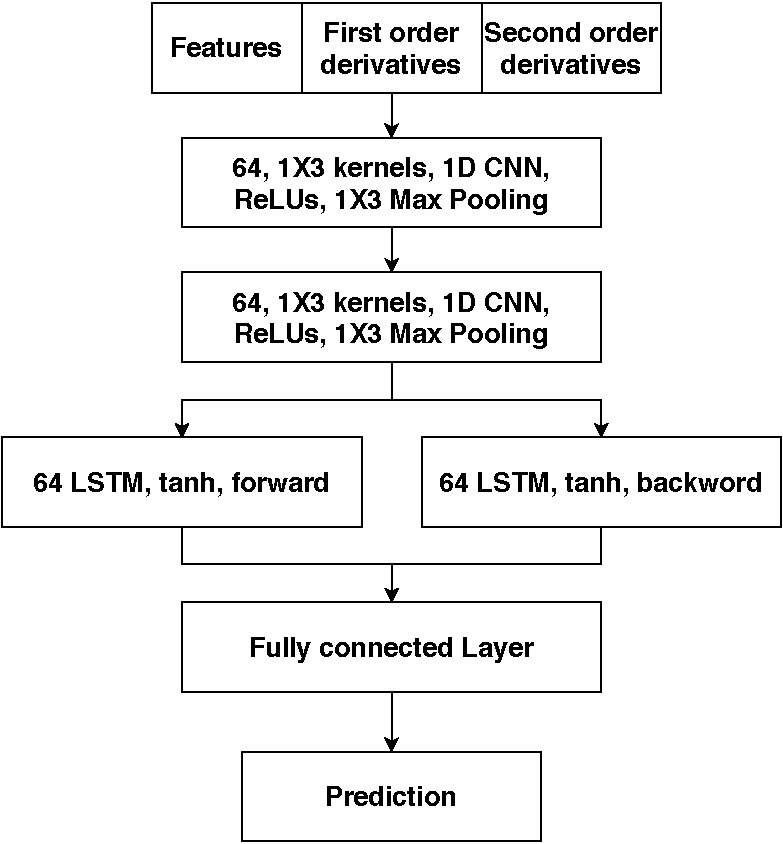
\includegraphics[width=\linewidth]{jagp2.pdf}
	\caption{A boat.}
	\label{fig1}
\end{figure}
\begin{figure}
	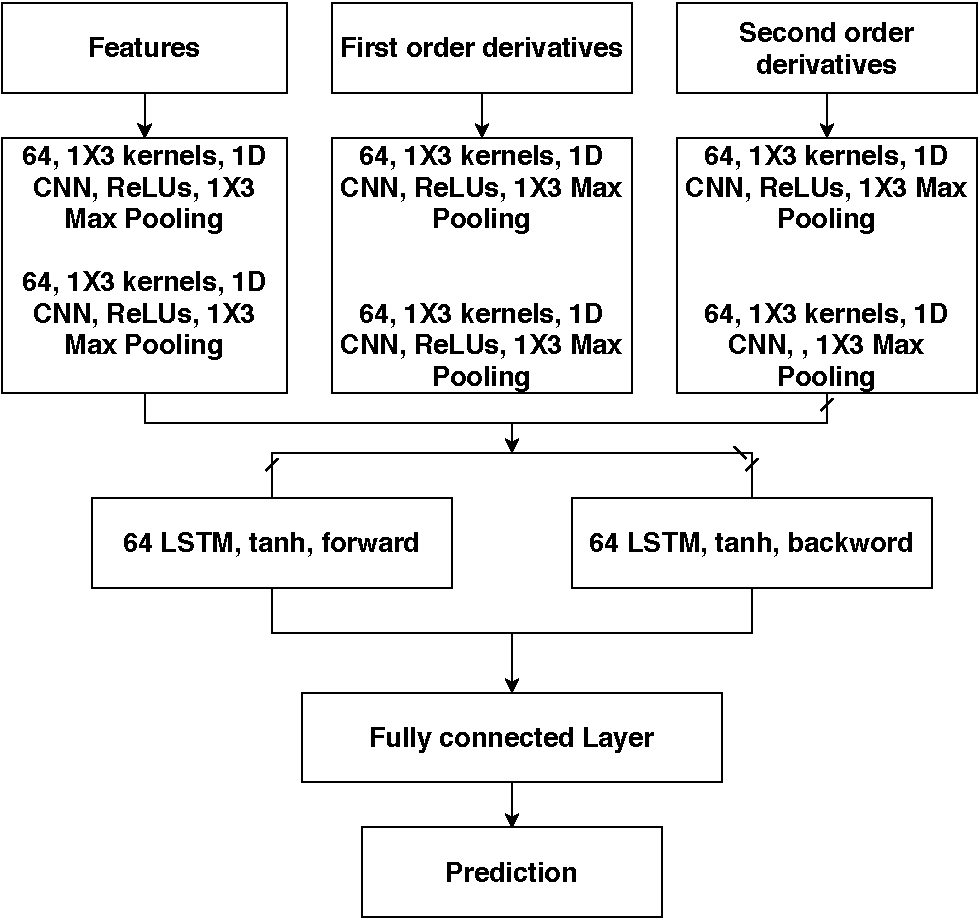
\includegraphics[width=\linewidth]{jagp.pdf}
	\caption{A boat.}
	\label{fig2}
\end{figure}
The proposed network intrusion detection system consists of two stages. One is fusion feature generation and another is the design of CBRNN architecture. Each stage is explained below in brief.
\subsection{Generation of fusion features}
The input dataset of network intrusion is a combination of different features of the form discrete, continuous and categorical values with varying ranges and resolution. Even a few features of the dataset may be null or infinite. Current machine learning/deep learning algorithms are not compatible with such data types. Hence, the dataset is preprocessed first to get significant features suitable for classification. Further, first and second-order derivates are computed from preprocessed features of size $M\times N$ using (\ref{eq1}) and (\ref{eq2}).
\begin{equation}
d_{m} =
\begin{cases}
c_{m+1}-c_{m} & \text{if $m=1$ }\\
c_{m}-c_{m-1} & \text{otherwise}
\end{cases}   
\label{eq1}    
\end{equation}
\begin{equation}
a_{m} =
\begin{cases}
d_{m+1}-d_{m} & \text{if $m=1$ }\\
d_{m}-d_{m-1} & \text{otherwise}
\end{cases}   
\label{eq2}    
\end{equation}
The first ($d_m$) and second-order ($a_m$) derivative features are also known as delta and delta-delta (acceleration) features respectively and widely used as supplementary features in speech/speaker recognition tasks. Preprocessed features and their first and second-order derivatives are fused (concatenated) to get fusion features.
\subsection{Convolutional Bidirectional Recurrent Neural Network}
Two CBRNN architectures of the proposed work are given in Figure~\ref{fig1} and \ref{fig2}. Both the architectures consist of one 1D CNN layer followed by Relu activation function and 1D max-pooling operation. The output of the CNN layer is fed as input to a bidirectional LSTM layer, the output of the bidirectional LSTM is input to the fully connected output layer with a sigmoid or softmax activation function. 
Each layer of CBRNN architecture is explained below in brief.
\subsubsection{CNN layer}
In this work, there are two ways are proposed to consider input to the CNN: preprocessed features and their first and second-order statistics are fused to get features of size $M\times N\times 3$ and fed as input to the CNN of CBRNN. This fusion is also known as early fusion. In another case, preprocessed features and their first and second-order statistics of sizes $M\times N\times 1$ are fed as input to the three separate CNNs. The outputs of these CNNs are fused and fed as input to the RNN. This fusion is also known as late fusion. 

\begin{table}
	\scriptsize
	\centering
	\caption{Confusion matrix of all categories over the UNSW-NB15 dataset with features and First Derivative of Features using Early Fusion classifier.}
	\makebox[\linewidth]{
		\begin{tabular}{|c|c|c|c|c|c|c|c|c|c|c|c|}	
			\hline
			Actual & \multicolumn{10}{c|}{Predicted} & \\
			\hline
			\hline
			 & Normal & Generic & Exploits & Analysis & Backdoor & DoS & Fuzzers & Reconn & Shellcode & Worms & Recall()\\
			\hline
			Normal & \textbf{24735} & 1 & 3574 & 8 & 0 & 6 & 7714 & 851 & 111 & 0 & 0.67\\
			\hline
			Generic & 148 & \textbf{18146} & 403 & 0 & 0 & 12 & 149 & 10 & 3 & 0 & 0.96\\
			\hline
			Exploits & 1019 & 0 & \textbf{9114} & 0 & 0 & 17 & 906 & 63 & 13 & 0 & 0.82 \\
			\hline
			Analysis & 16 & 0 & 658 & \textbf{1} & 0 & 0 & 2 & 0 & 0 & 0 & 0.00 \\
			\hline
			Backdoor & 15 & 0 & 544 & 0 & \textbf{4} & 0 & 18 & 2 & 0 & 0 & 0.01\\
			\hline
			DoS & 215 & 6 & 3460 & 0 & 0  & \textbf{75} & 308 & 22 & 3 & 0 & 0.02\\
			\hline
			Fuzzers & 753 & 0 & 1914  & 0 & 0 & 4 & \textbf{3104} & 256 & 31 & 0 & 0.51\\	
			\hline
			Reconn & 34 & 4 & 726 & 0 & 0 & 6 & 253 & \textbf{2473} & 0 & 0 & 0.71\\
			\hline
			Shellcode & 20 & 6 & 91 & 0 & 0 & 2 & 187 & 26 & \textbf{46} & 0 & 0.12\\
			\hline
			Worms & 6 & 0 & 34 & 0 & 0 & 0 & 4 & 0 & 0 & \textbf{0} & 0.00\\
			\hline	
			Precision() & 0.92 & 1.00 & 0.44 & 0.11 & 1.00 & 0.61 & 0.25 & 0.67 & 0.22 & 0.00 \\
			\hline
		\end{tabular}
	}
	\label{table1}
\end{table}

\begin{table}
	\scriptsize
	\centering
	\caption{Performance of our proposed methods for Binary Classification using the UNSW-NB15 Dataset.}
	\begin{tabular}{|c|c|c|c|}
		\hline
		Method & Order of Derivative & Training Accuracy & Validation Accuracy\\
		\hline
		\hline
		Early Fusion & First & 89.24 & 75.67\\	
		\hline
		 & Second & 91.04 & 78.58\\
		\hline
		\hline
		Late Fusion & First & 88.07 & 75.63\\
		\hline
		 & Second & 89.67 & 76.54\\
		\hline	
	\end{tabular}
	
	\label{table2}
\end{table}

\begin{table}
	\scriptsize
	\centering
	\caption{Performance of our proposed methods for Multiclass Classification using the UNSW-NB15 Dataset.}
	\begin{tabular}{|c|c|c|c|c|c|c|}
		\hline
		Method & Order of Derivative & Accuracy & Precision & Recall & F1-score\\
		\hline
		\hline
		Early Fusion & First & 70.08 & 0.79 & 0.70 & 0.71 \\	
		\hline
		\hline
		Late Fusion & First & 62.10 & 0.72 & 0.62 & 0.63\\
		\hline	
	\end{tabular}
	\label{table3}
\end{table}

\section{Bibliography styles}

There are various bibliography styles available. You can select the style of your choice in the preamble of this document. These styles are Elsevier styles based on standard styles like Harvard and Vancouver. Please use Bib\TeX\ to generate your bibliography and include DOIs whenever available.

Here are two sample references: \cite{Feynman1963118,Dirac1953888}.

\section*{References}

\bibliography{mybibfile}

\end{document}